% Compatibility: if the main document uses the \texttt{article} class, \chapter is undefined.
\providecommand{\chapter}[1]{\section{#1}}
\chapter{Mid-Term Progress and Results}
\label{ch:mid-term-progress}

This chapter summarizes the development progress achieved up to the mid-term milestone for the proposed \textit{Automated Two-Wheeler Violation Detection and E-Challan System}. The work completed so far covers the core computer-vision pipeline (vehicle/rider detection, helmet compliance classification, and preliminary ANPR/OCR), along with initial backend services and a role-based dashboard interface intended for operational monitoring and administrative verification.

\section{Work Completed So Far}
\label{sec:work-completed}

\subsection{Machine Learning Models Development}
\label{subsec:ml-models-development}

\subsubsection{Vehicle Detection (Motorcycle Localization)}
A YOLOv8-based object detection model has been configured and trained to localize two-wheelers in surveillance frames by producing bounding boxes around motorcycles. The current detection pipeline includes frame extraction, inference-time pre-processing, confidence thresholding, and post-processing for bounding box filtering. This module serves as the primary trigger for downstream analytics by defining the region-of-interest for rider association, helmet inspection, and number plate localization.

\subsubsection{Helmet Detection (Helmet vs. No Helmet Classification)}
A dedicated helmet compliance module has been implemented using a classification model that categorizes detected riders into \textit{Helmet} and \textit{No Helmet}. The workflow follows a two-stage strategy: (i) localize rider instances from the two-wheeler context and (ii) crop rider head/upper-body regions for classification. The module outputs predicted class labels and confidence scores which are subsequently consumed by the violation decision logic.

\subsubsection{Number Plate Detection and Recognition (ANPR and OCR Extraction)}
A preliminary Automatic Number Plate Recognition (ANPR) workflow has been implemented to extract vehicle registration numbers from evidence frames. The current pipeline performs (i) number plate localization on candidate frames and (ii) text extraction using EasyOCR/PaddleOCR. Post-OCR cleaning rules have been introduced to normalize the extracted strings (e.g., removal of spurious symbols and whitespace) and to retain a confidence measure that can be used for manual verification within the dashboard.

\subsection{Backend and Frontend Infrastructure}
\label{subsec:backend-frontend}

\subsubsection{Role-Based Access Control (RBAC)}
A role-based access control (RBAC) mechanism has been established to separate system privileges across two primary operator roles: \textit{Admin} and \textit{Traffic Police}. The Admin role is responsible for configuration and user management (e.g., onboarding, role assignment, and system settings), whereas the Traffic Police role is focused on operational verification, evidence review, and challan approval decisions. Authentication and authorization have been designed to be enforced consistently across API endpoints and UI routes.

\subsubsection{E-Challan Module (Digital Challan Generation Logic)}
An initial e-challan generation module has been implemented to translate validated violations into structured challan records. The module supports generation of unique challan identifiers, mapping of violation types to fine definitions, and storage of timestamps and evidence references. The current implementation is designed to integrate with a human-in-the-loop verification process whereby Traffic Police confirm or reject suggested challans based on captured evidence.

\subsubsection{Frontend Dashboard (Monitoring and Administration UI)}
A React-based dashboard has been developed to provide an operational interface for monitoring detected events and performing administrative actions. The dashboard includes role-based views, violation listing, evidence preview, and basic search/filter utilities (e.g., by plate number and time). The UI design emphasizes rapid evidence inspection and decision-making while maintaining auditability through structured records.

\section{Preliminary Results and System Interface}
\label{sec:preliminary-results}

\subsection{Preliminary Model Performance Outputs}
\label{subsec:preliminary-model-performance}

The preliminary training and validation outputs indicate that the detection and classification modules are functioning as intended for mid-term evaluation. The following figures summarize current training behavior and initial diagnostic metrics; these results are treated as intermediate and will be strengthened through expanded datasets, additional augmentation, and iterative hyperparameter tuning.

The model results visualization in Figure~\ref{fig:helmet-model-results} provides a consolidated view of training dynamics (e.g., learning progression and metric stabilization). It is primarily used to confirm convergence trends and to detect overfitting/underfitting patterns that may require adjustments in data balancing or training schedules.
\begin{figure}[htbp]
    \centering
    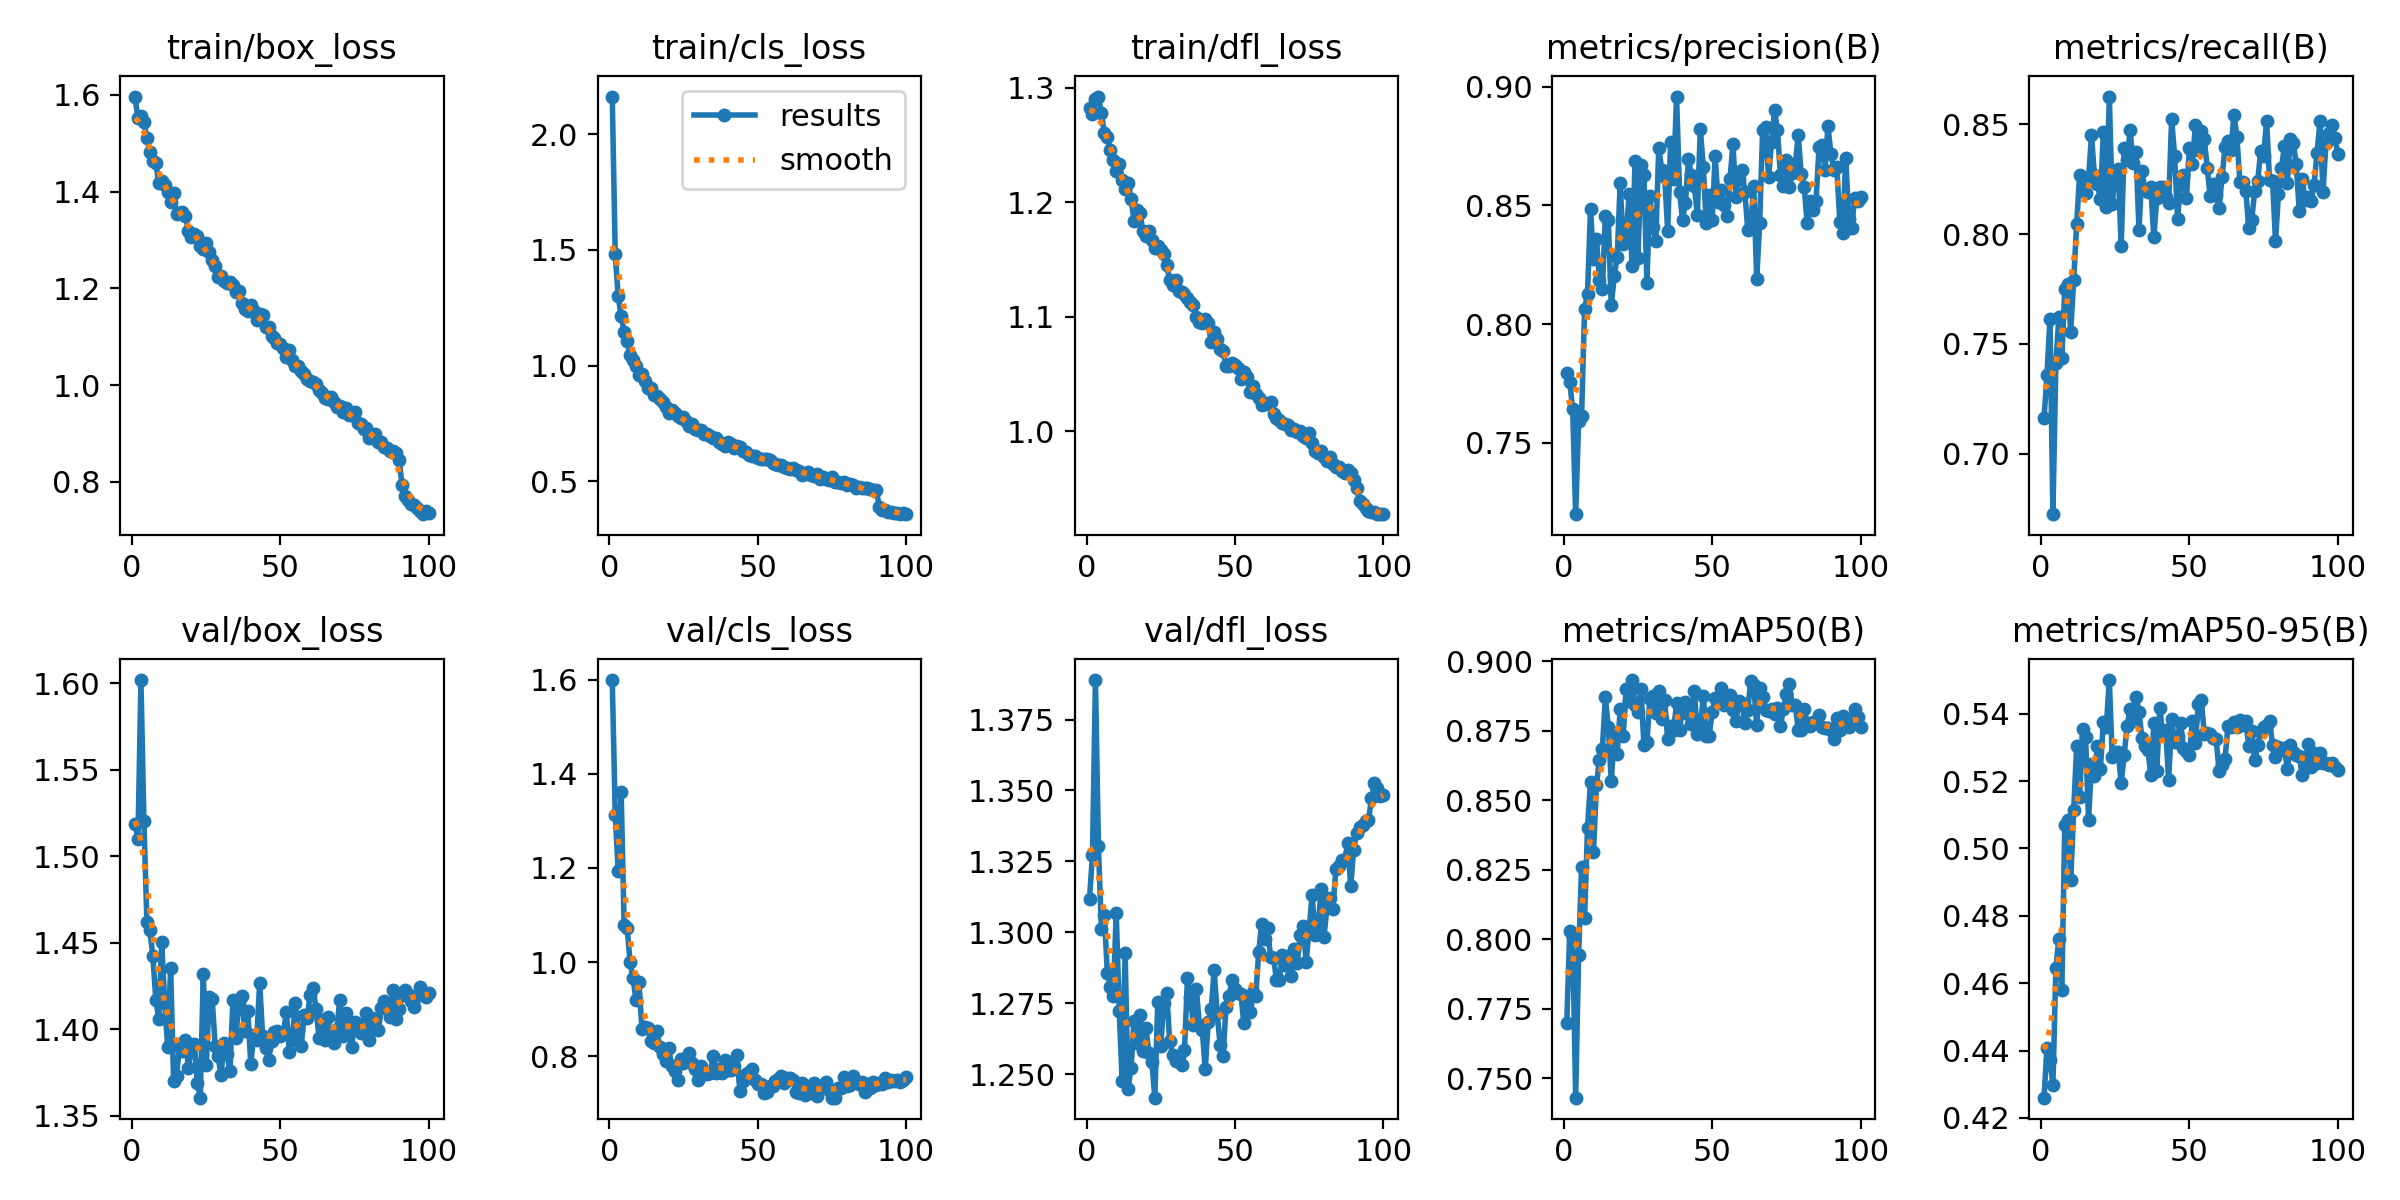
\includegraphics[width=0.8\textwidth]{figures/model_results/helmet_model_results.png}
    \caption{Training summary for the helmet compliance model.}
    \label{fig:helmet-model-results}
\end{figure}

The precision--recall (PR) curve in Figure~\ref{fig:pr-curve} characterizes the trade-off between precision and recall across confidence thresholds. This diagnostic is used to select operational thresholds appropriate for enforcement settings, where false positives must be controlled while maintaining adequate recall for safety-critical violations.
\begin{figure}[htbp]
    \centering
    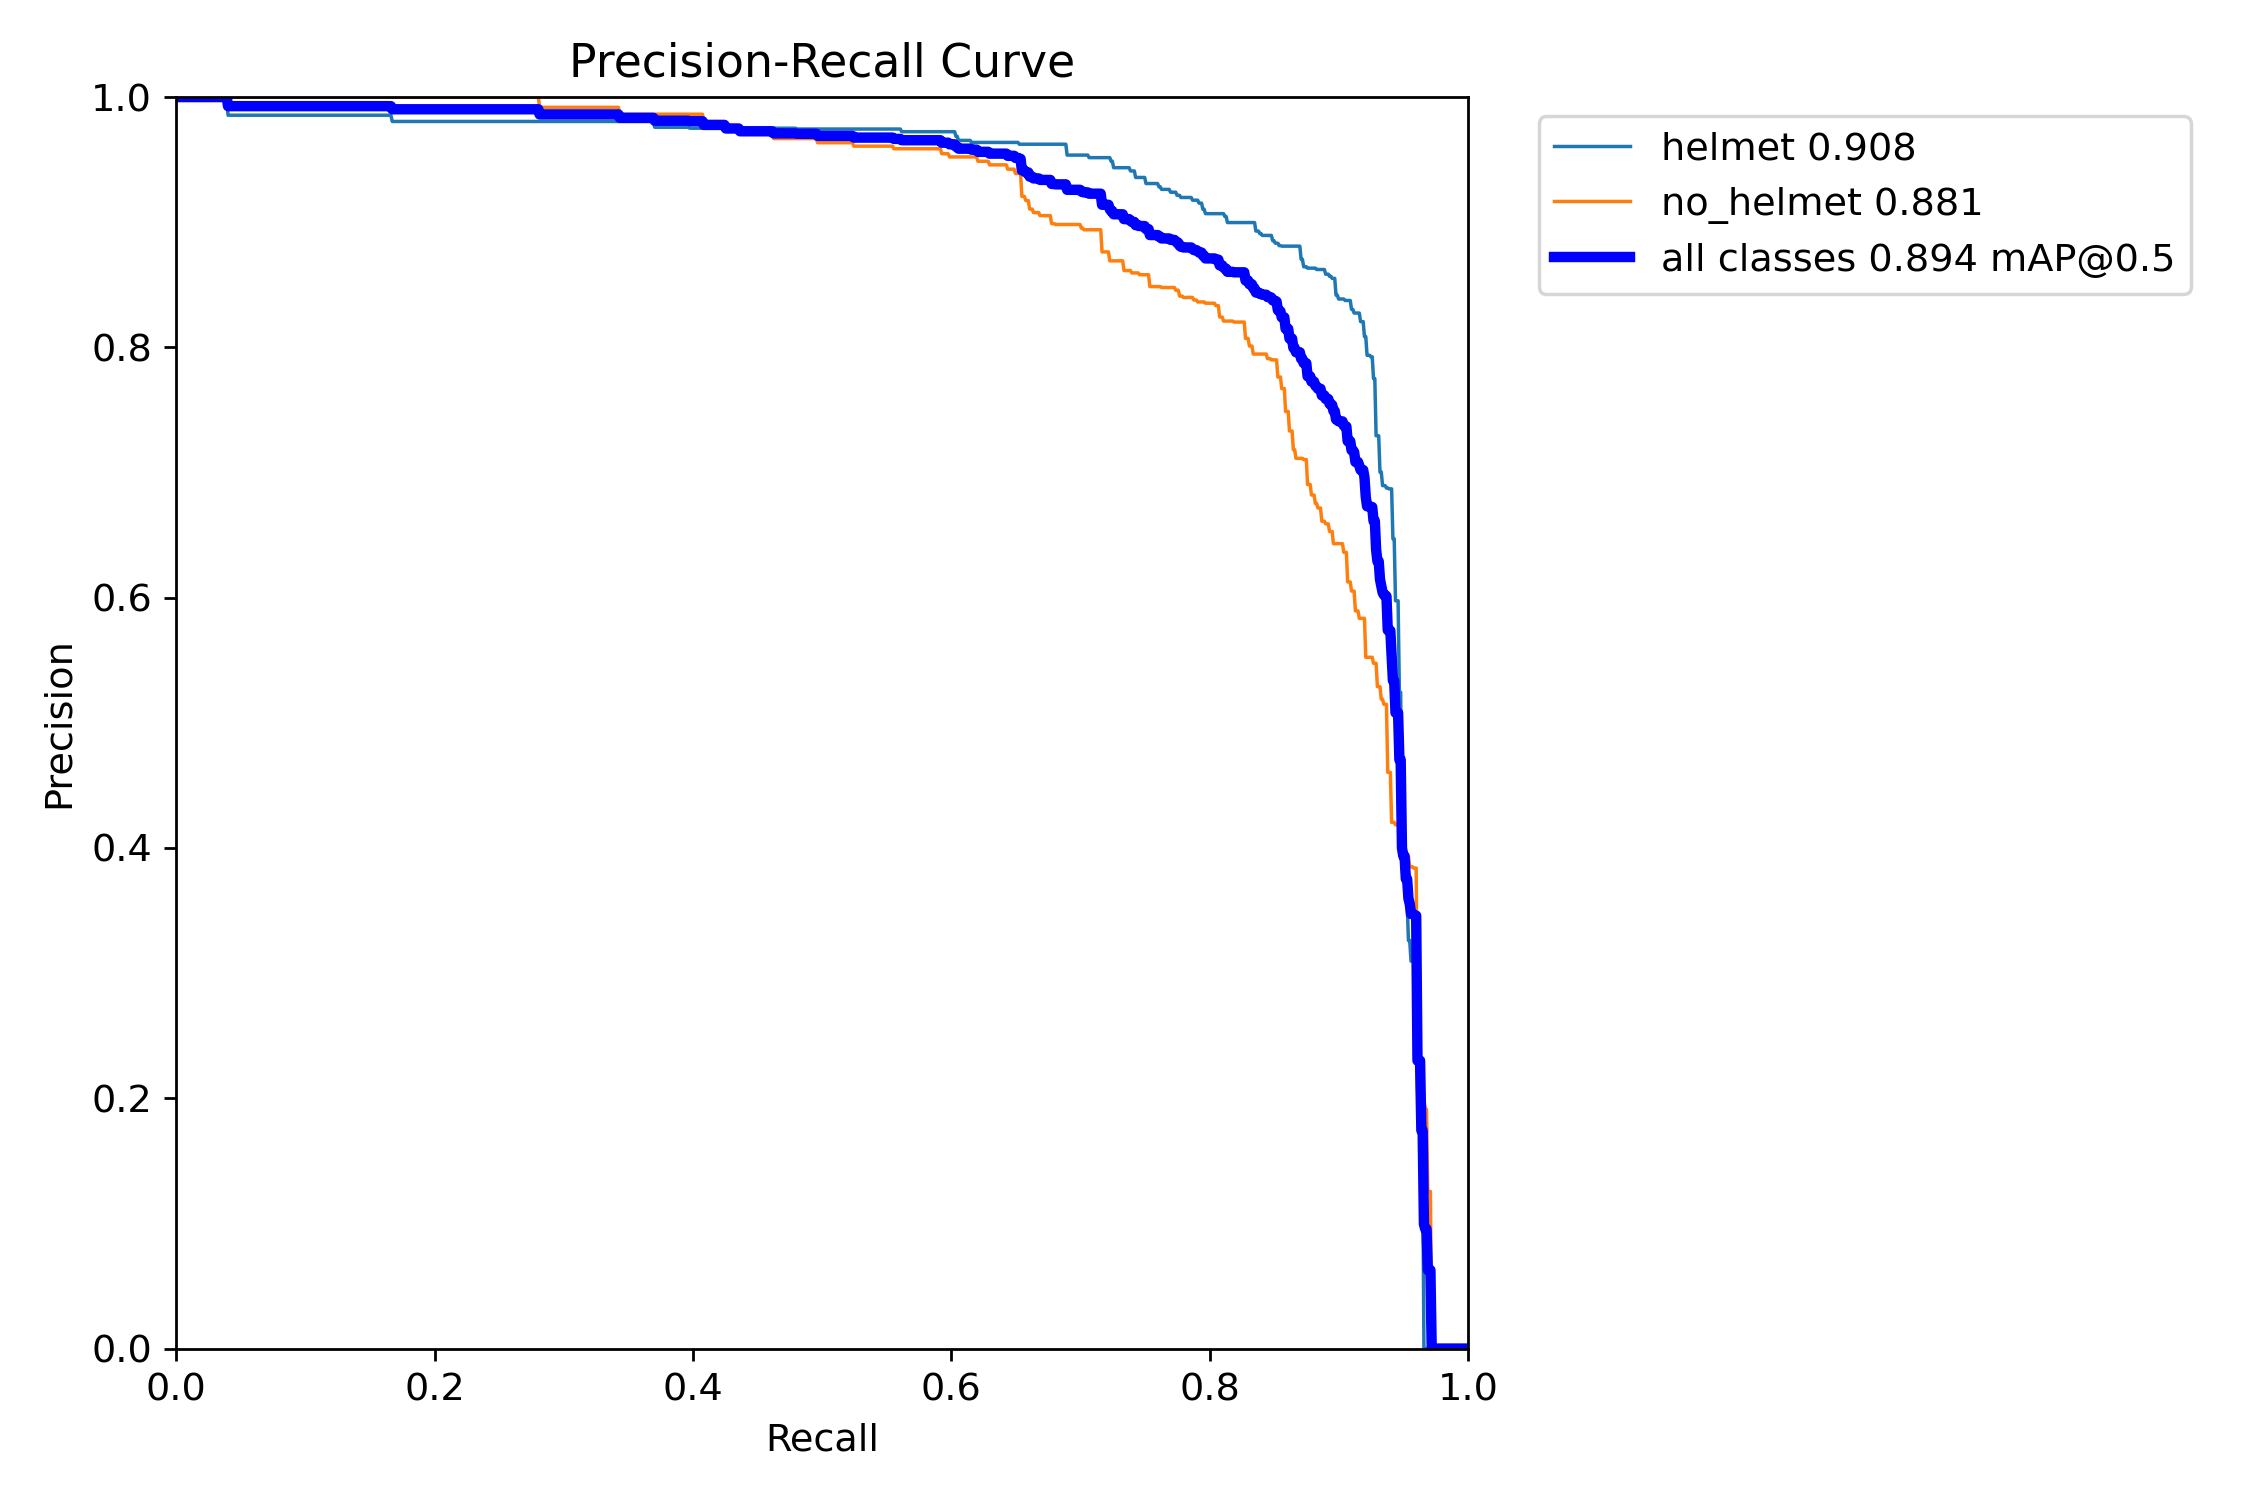
\includegraphics[width=0.8\textwidth]{figures/model_results/Helmet_BoxPR_curve.png}
    \caption{Precision--recall curve for the trained detection/classification pipeline (intermediate).}
    \label{fig:pr-curve}
\end{figure}

The confusion matrix in Figure~\ref{fig:confusion-matrix} presents class-wise error distribution and provides insight into systematic misclassifications (e.g., confusion between visually similar classes due to occlusion, motion blur, and small object scale). These observations directly inform dataset refinement and targeted augmentation strategies.
\begin{figure}[htbp]
    \centering
    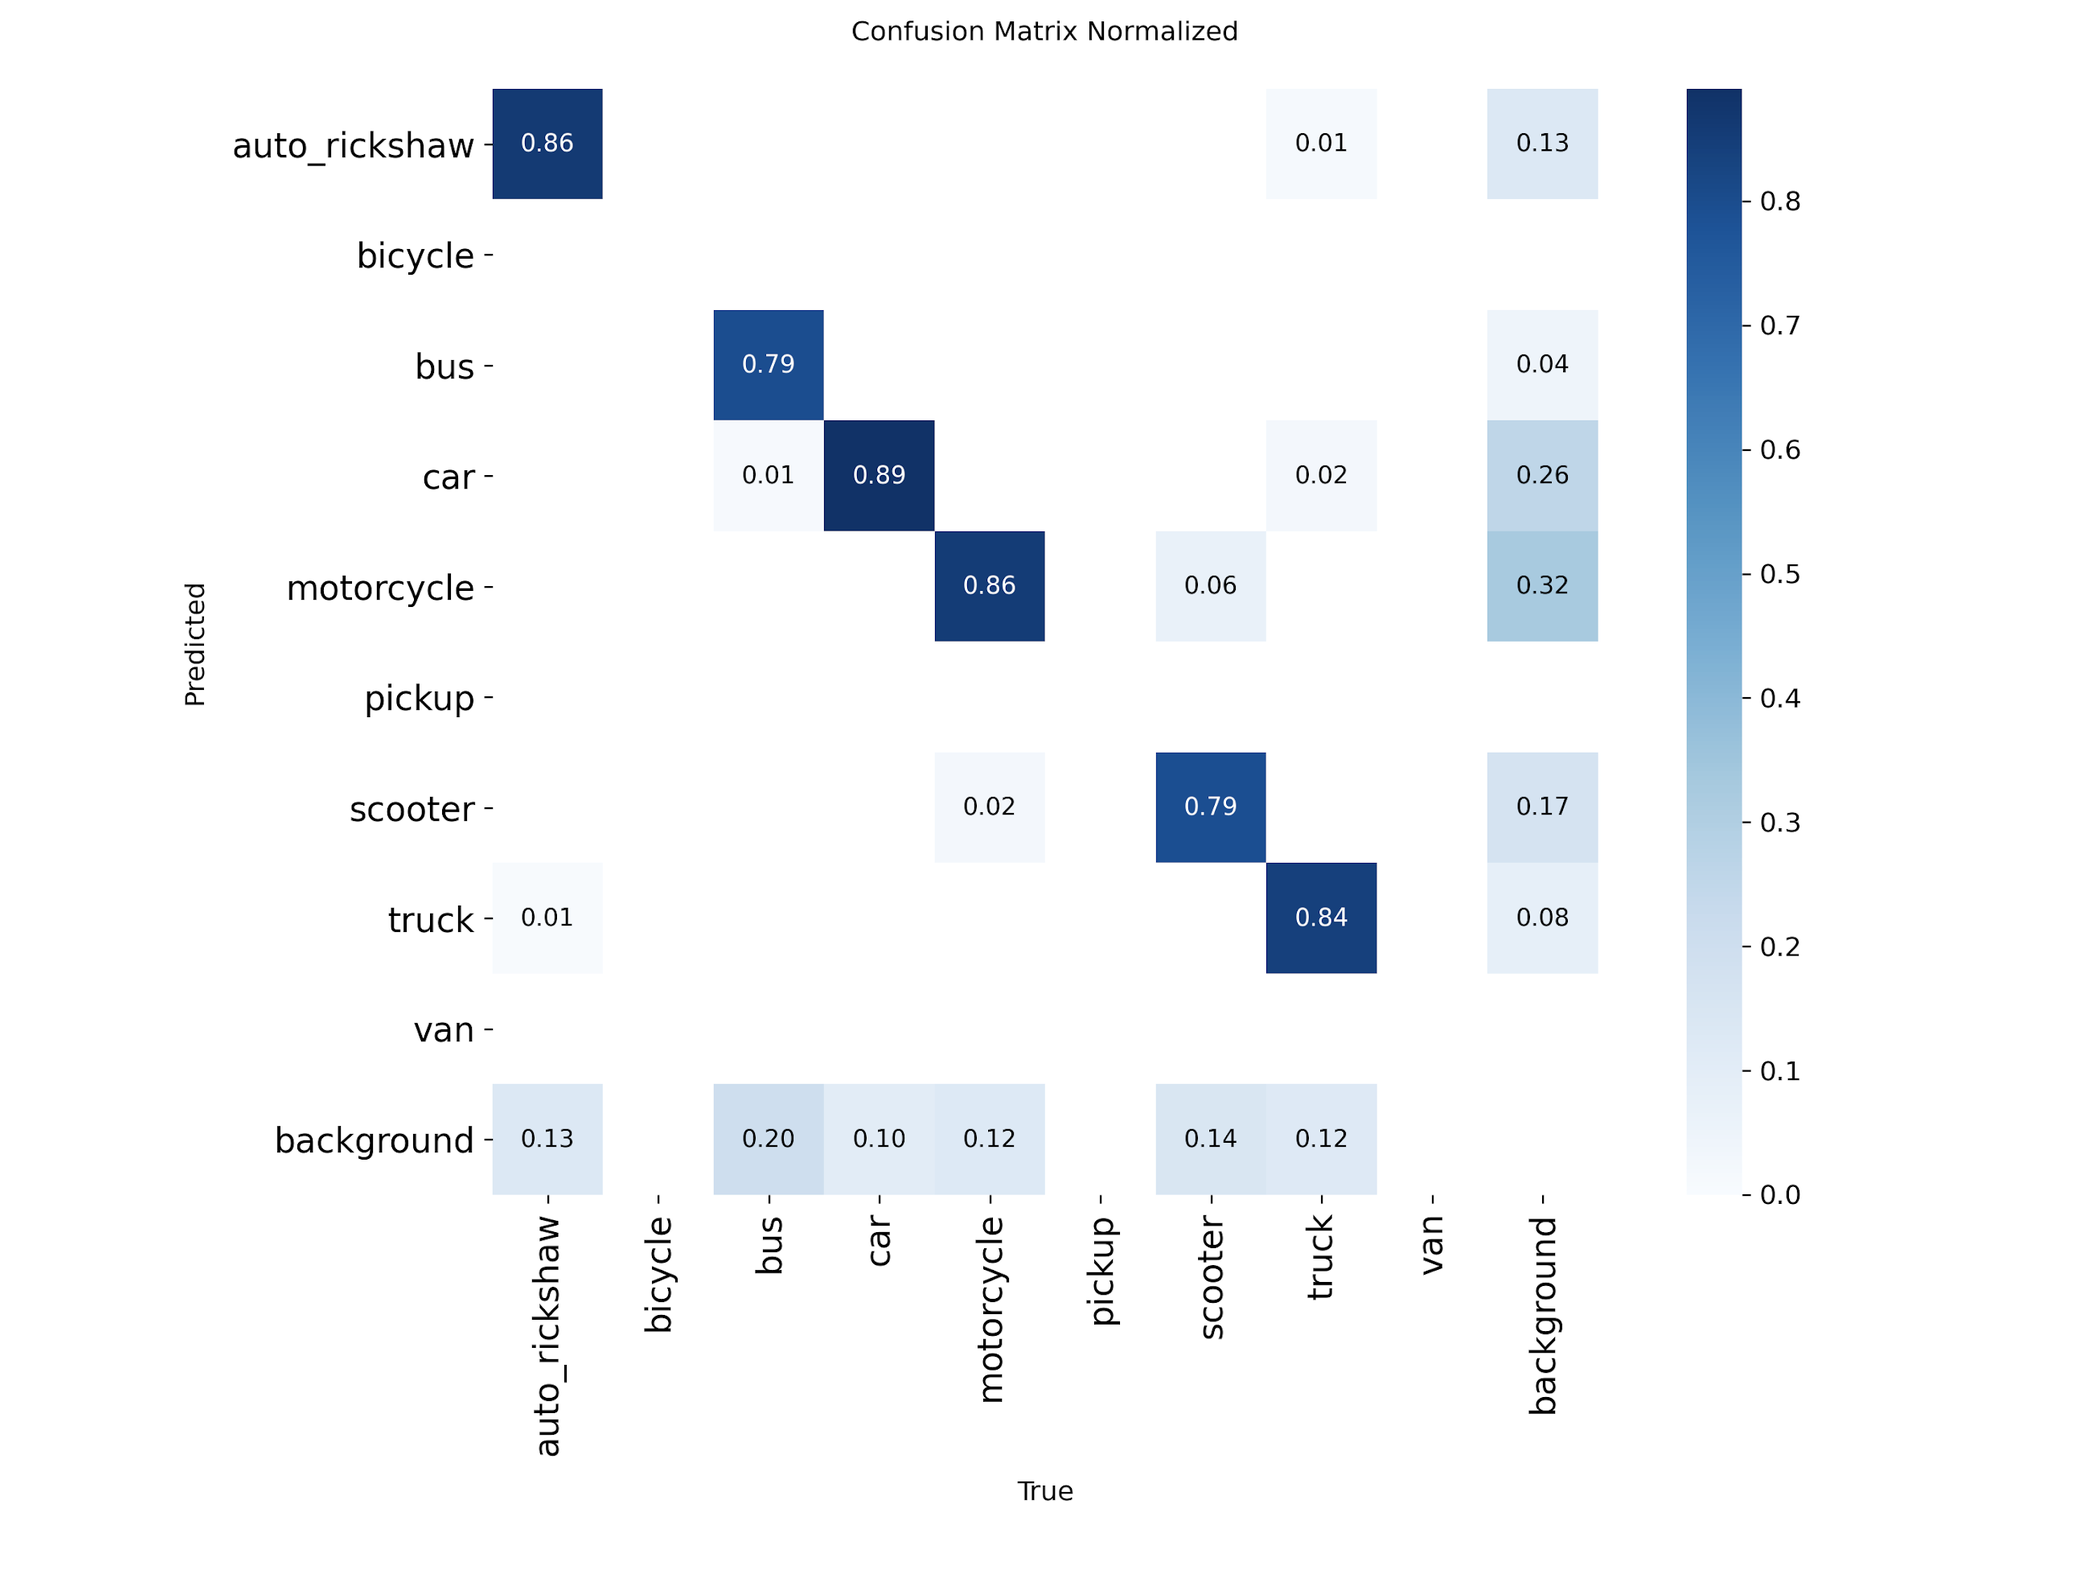
\includegraphics[width=0.8\textwidth]{figures/model_results/normalized_confusion_vehicle_detect.png}
    \caption{Normalized confusion matrix for the current vehicle detection model (intermediate).}
    \label{fig:confusion-matrix}
\end{figure}

\subsection{Preliminary System Interface Views}
\label{subsec:preliminary-system-interface}

Figure~\ref{fig:admin-view} demonstrates the Admin interface used to manage users, configure system parameters, and monitor operational status at a high level. This view supports governance and access management to ensure that only authorized personnel can approve enforcement actions or modify core system settings.
\begin{figure}[htbp]
    \centering
    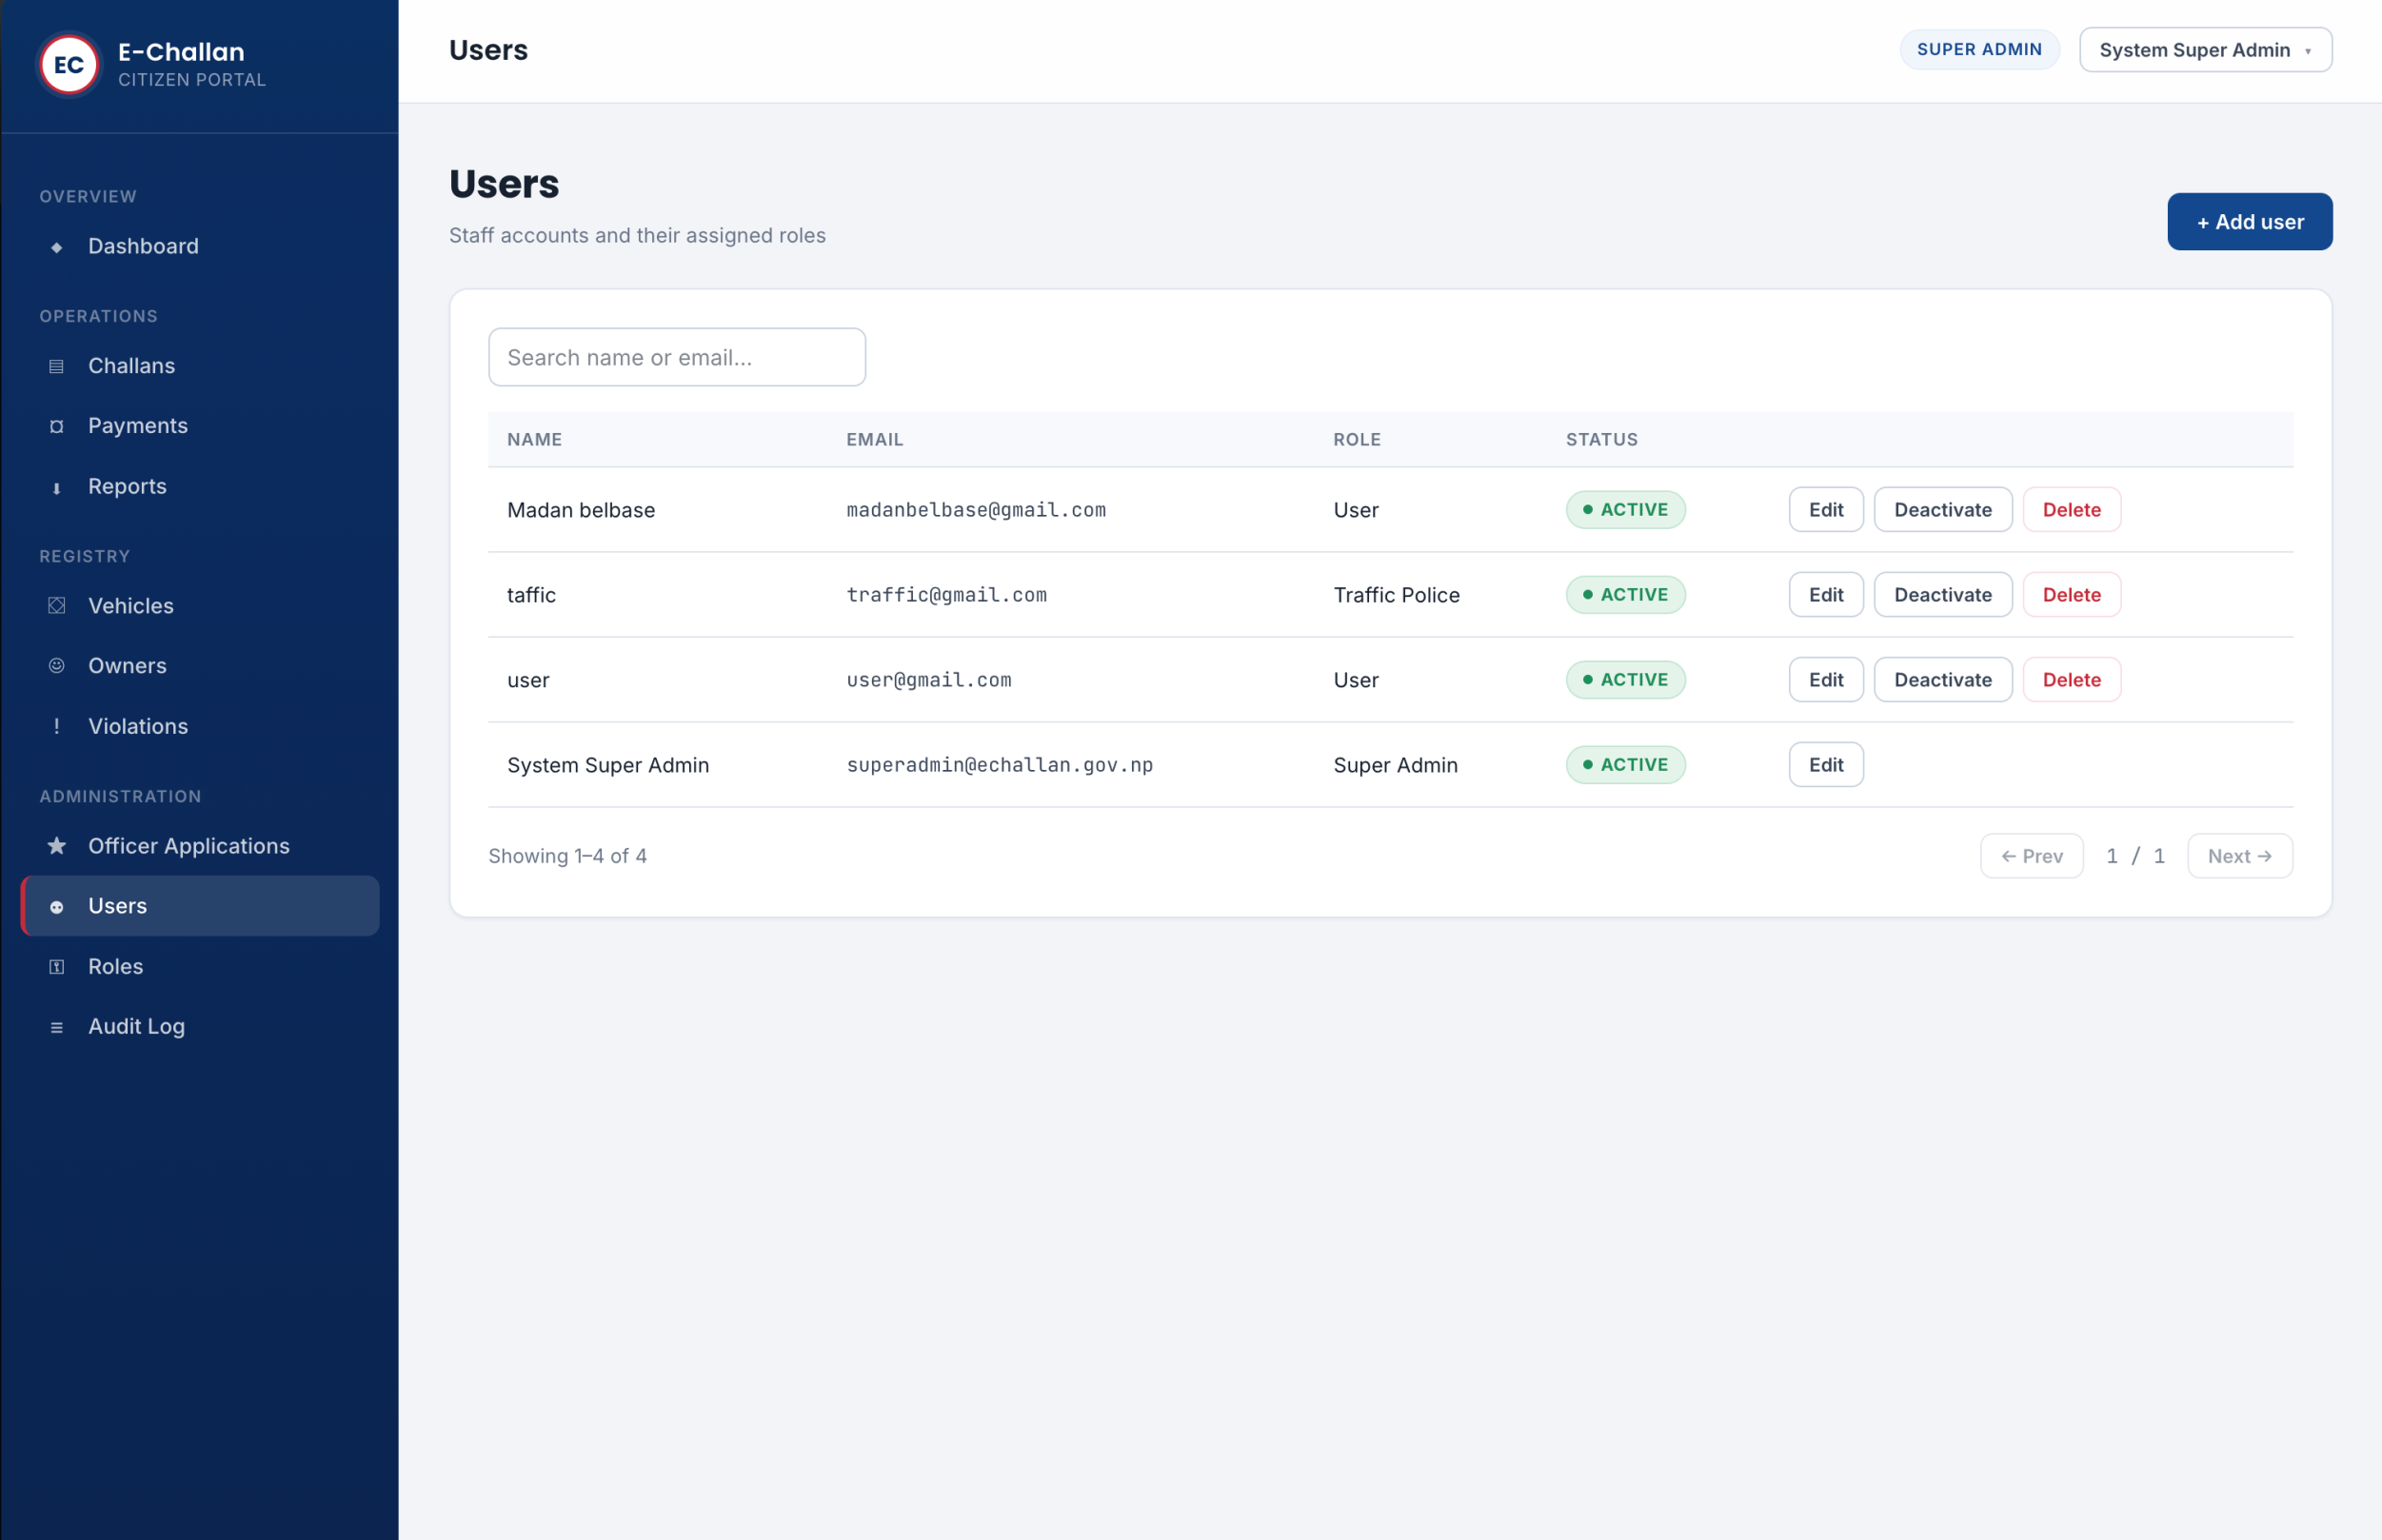
\includegraphics[width=0.8\textwidth]{figures/backend_frontend_figures/super_admin_manage_users.png}
    \caption{Role-based Admin view for user and system management.}
    \label{fig:admin-view}
\end{figure}

Figure~\ref{fig:traffic-officer-view} presents the Traffic Police interface designed for evidence verification, violation review, and challan approval. The layout prioritizes rapid decision-making by displaying essential metadata (time, location, violation type) alongside evidence media and verification actions.
\begin{figure}[htbp]
    \centering
    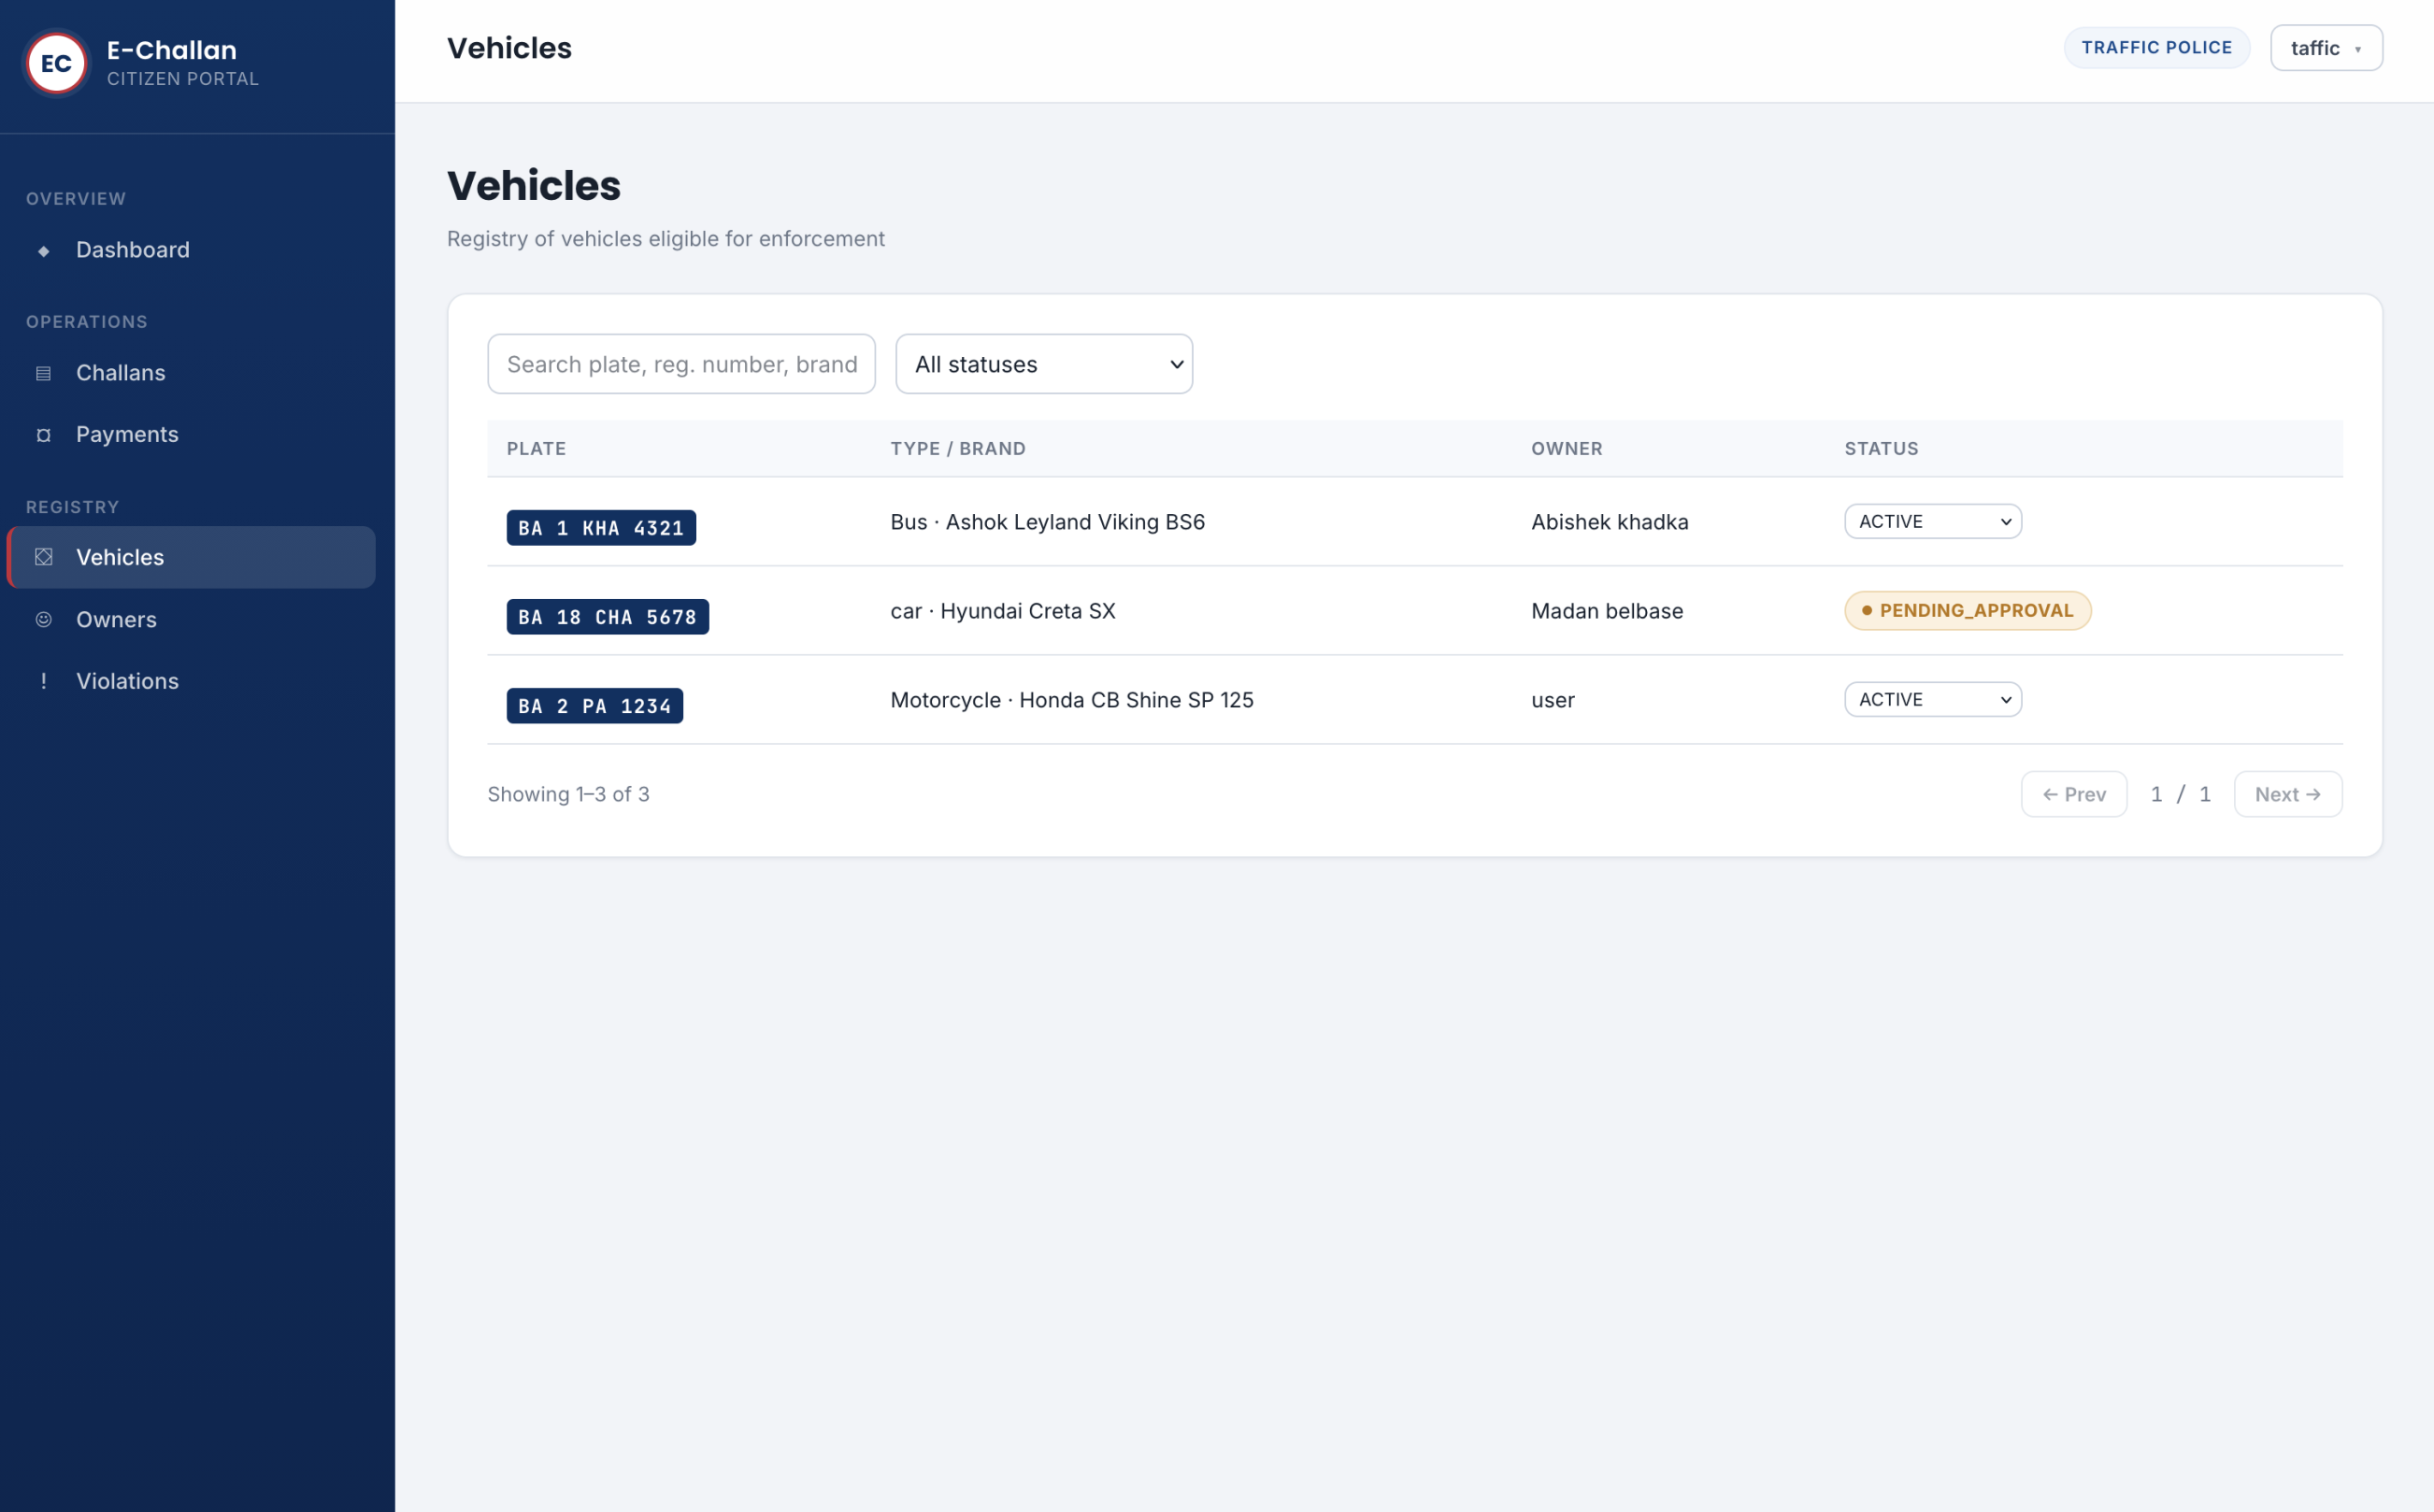
\includegraphics[width=0.8\textwidth]{figures/backend_frontend_figures/traffic_view.png}
    \caption{Traffic Police view for reviewing violations and validating e-challans.}
    \label{fig:traffic-officer-view}
\end{figure}

Figure~\ref{fig:user-view} shows the general user-facing dashboard concept, intended to provide transparent access to issued challans, violation history, and payment-related tracking. This interface supports accountability and reduces friction in fine settlement processes by centralizing challan details and evidence references.
\begin{figure}[htbp]
    \centering
    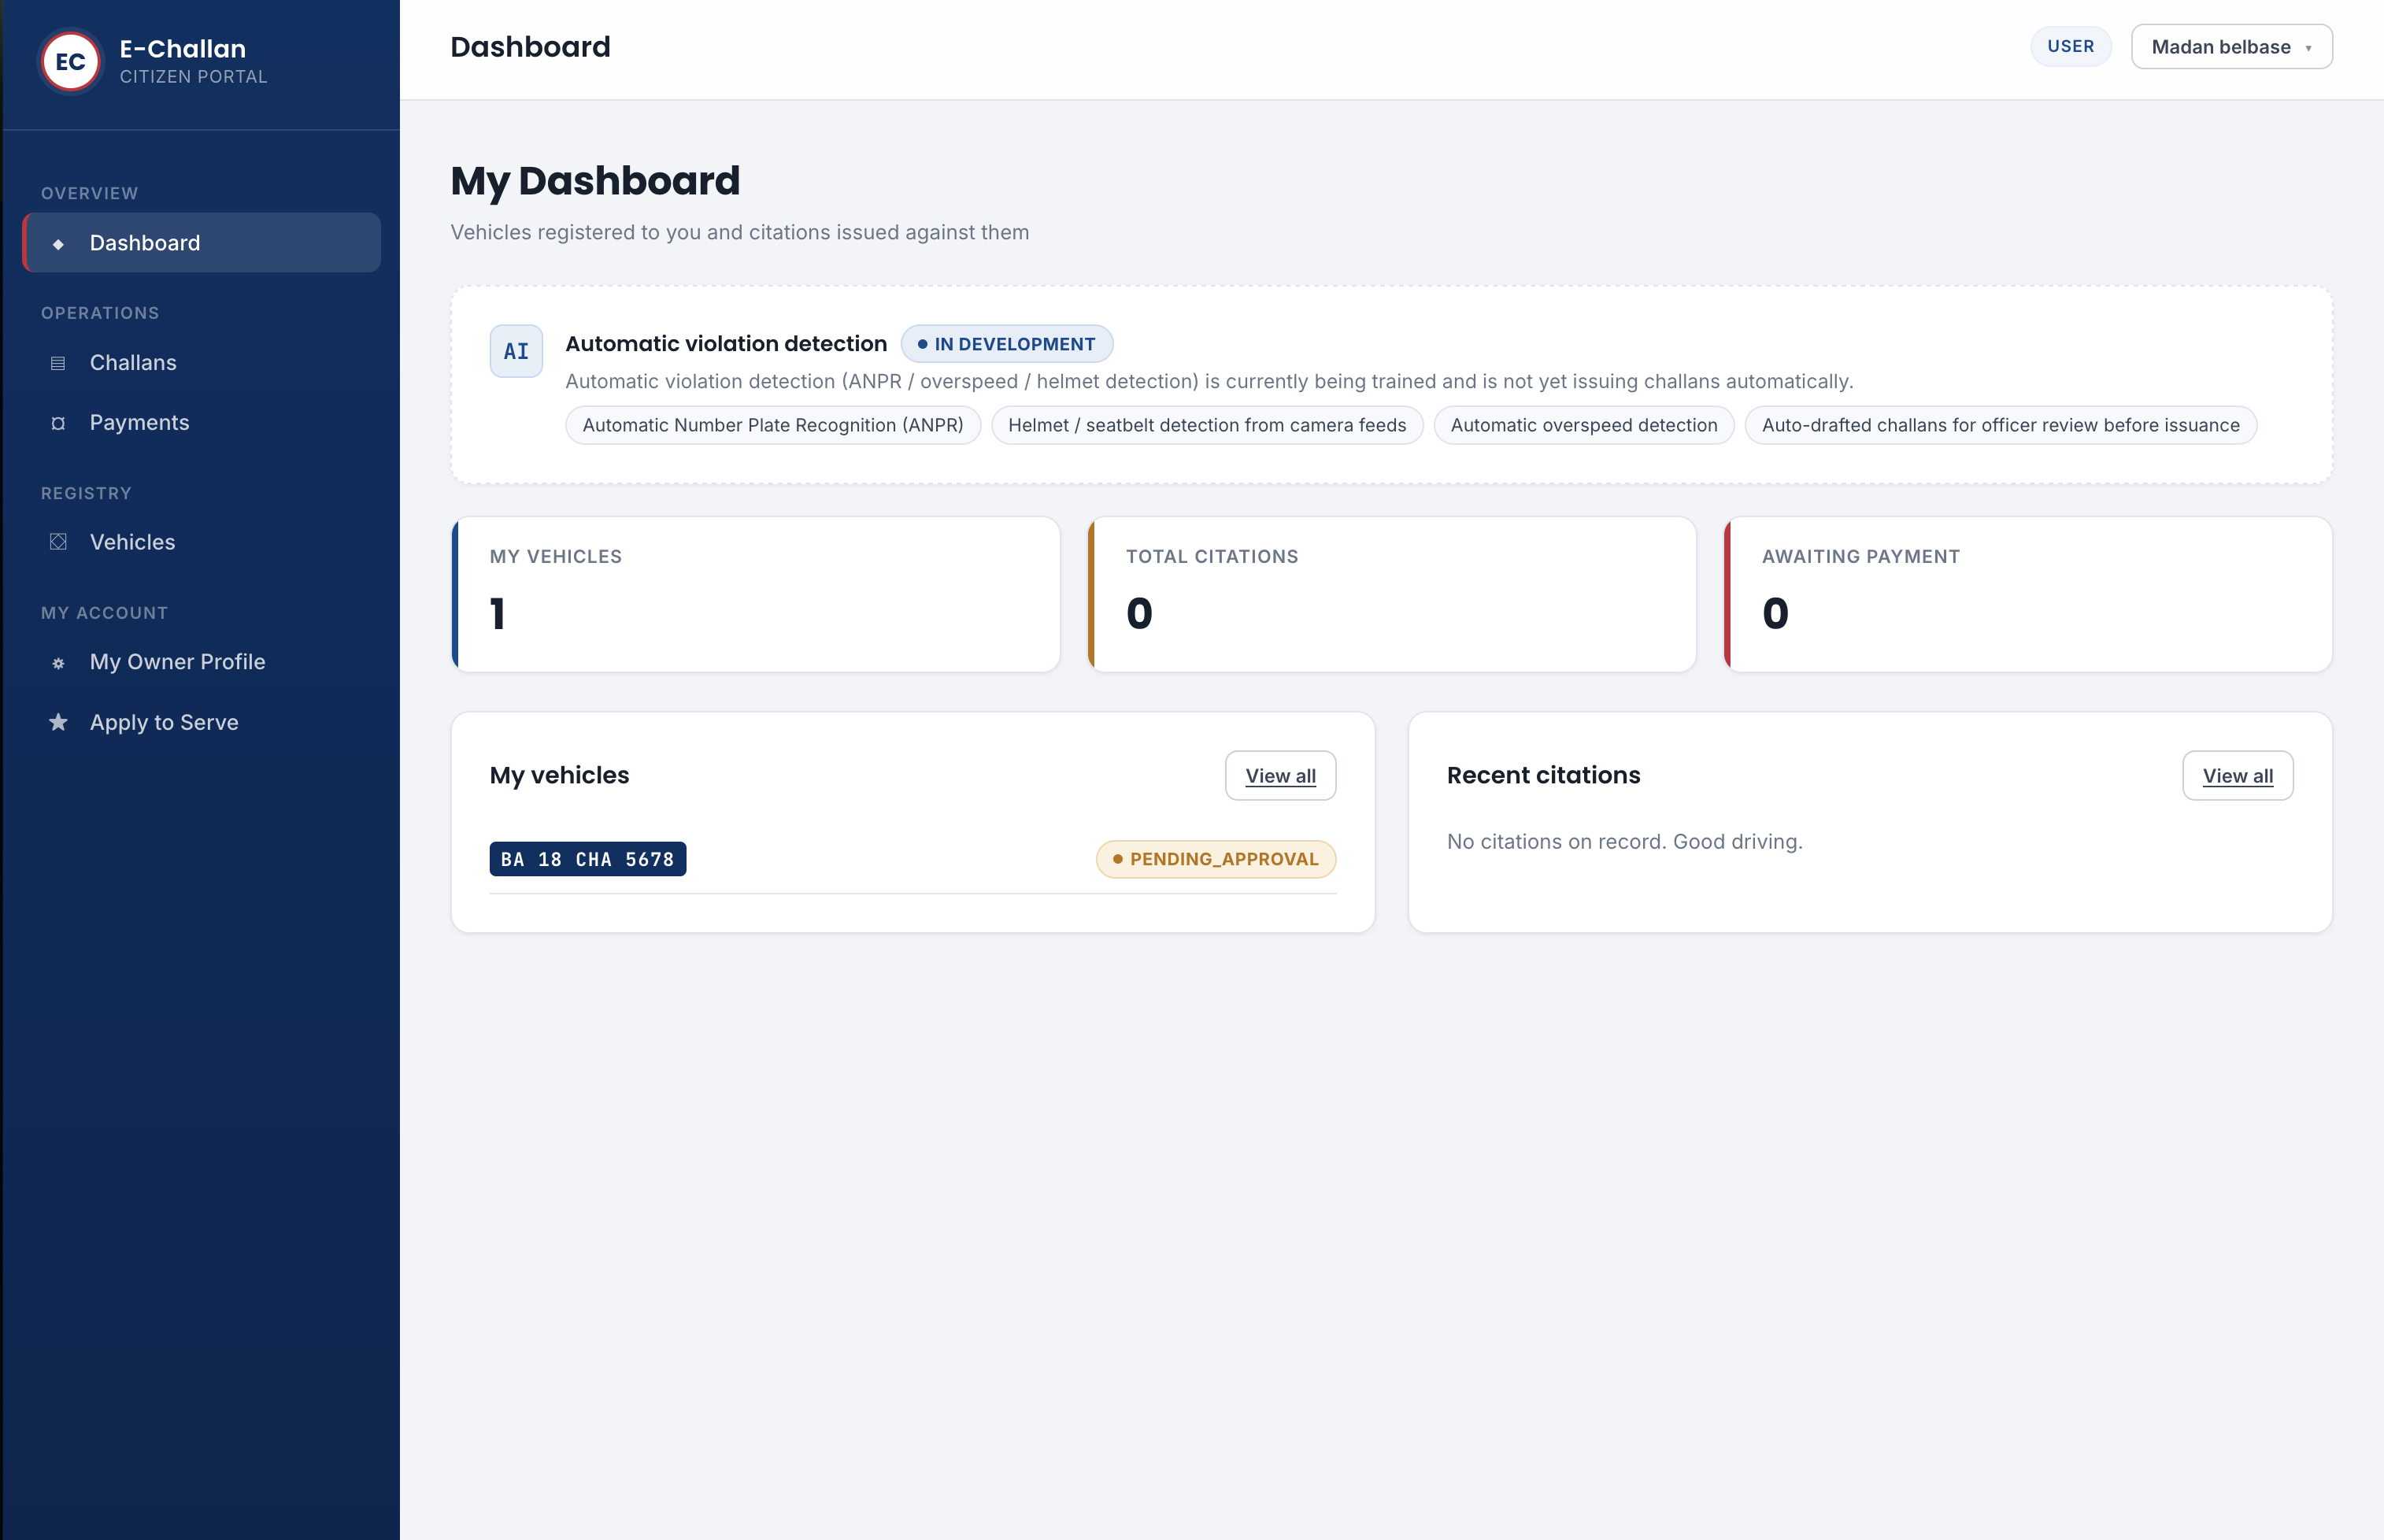
\includegraphics[width=0.8\textwidth]{figures/backend_frontend_figures/user_dashboard.png}
    \caption{General user view for challan history and fine tracking.}
    \label{fig:user-view}
\end{figure}

\section{Remaining Work}
\label{sec:remaining-work}

\subsection{System Integration}
\label{subsec:system-integration}
The final phase will prioritize end-to-end integration of the ML inference pipeline with the service layer and user interfaces. This includes connecting real-time inference outputs (detections, classifications, OCR strings, and confidence scores) to the FastAPI/Node.js backend, designing stable event payloads, implementing evidence storage workflows, and ensuring that the React dashboard receives real-time updates with consistent status transitions (e.g., \textit{Detected} $\rightarrow$ \textit{Pending Review} $\rightarrow$ \textit{Approved/Rejected} $\rightarrow$ \textit{Challan Issued}).

\subsection{Additional Model Training and Implementation}
\label{subsec:additional-models}
Two additional violation categories will be implemented to complete the multi-violation scope:
\begin{itemize}
    \item \textbf{Triple Riding Detection:} Extend the detection pipeline to associate multiple riders with each motorcycle and reliably estimate rider count under occlusions and varying camera angles.
    \item \textbf{Mobile Phone Usage Detection:} Train and deploy a specialized detector/classifier to identify handheld mobile usage by riders, accounting for small object size, motion blur, and partial occlusion.
\end{itemize}

\subsection{Mobile Application Development}
\label{subsec:mobile-app}
A lightweight mobile application will be developed to support on-the-go monitoring for authorized traffic personnel and fine tracking for vehicle owners. The planned application will integrate with the same backend APIs to provide authenticated access, notification support, and a streamlined interface for viewing violations, evidence media, and challan payment status.
\end{enumerate}